\section{Resultados}

\subsection{Seleção de Atributos por Filtragem}

\begin{figure}[h]
\centering
\caption{\label{figure:figura1}Seleção de Atributos Baseada em Filtragem com \textit{SelectKBest} \cite{b5}}
  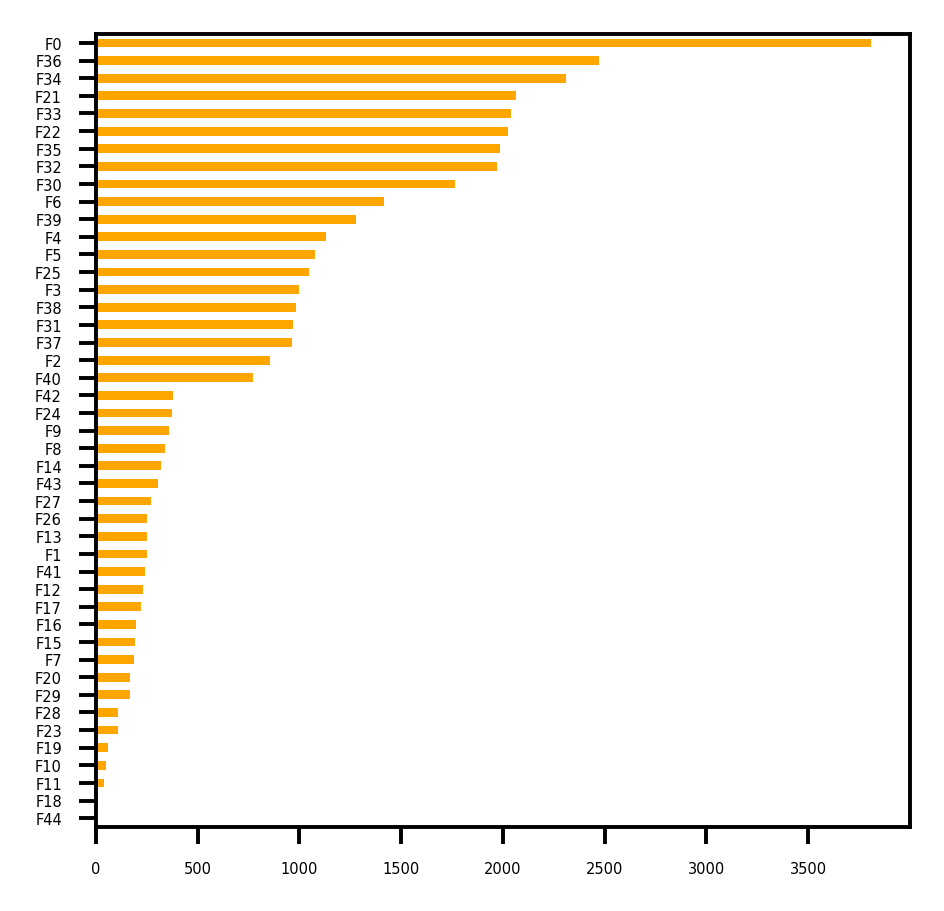
\includegraphics[width=0.45\textwidth,height=90mm]{assets/selectkbest.png}
  \\ Fonte: Condução dos experimentos pelos autores do artigo.
\end{figure}

\subsection{Seleção de Atributos com Base nos Modelos Testados}

Realizamos uma seleção de atributos com base nos modelos \textit{RandomForestClassifier}, \textit{XGBClassifier}, \textit{AdaBoostClassifier} e \textit{LGBMClassifier}, extraindo a média dos valores de \texttt{\footnotesize{feature\_importances\_}} dos modelos.

\begin{figure}[h]
\centering
\caption{\label{figure:figura2}Seleção de Atributos com Base nos Modelos Testados}
  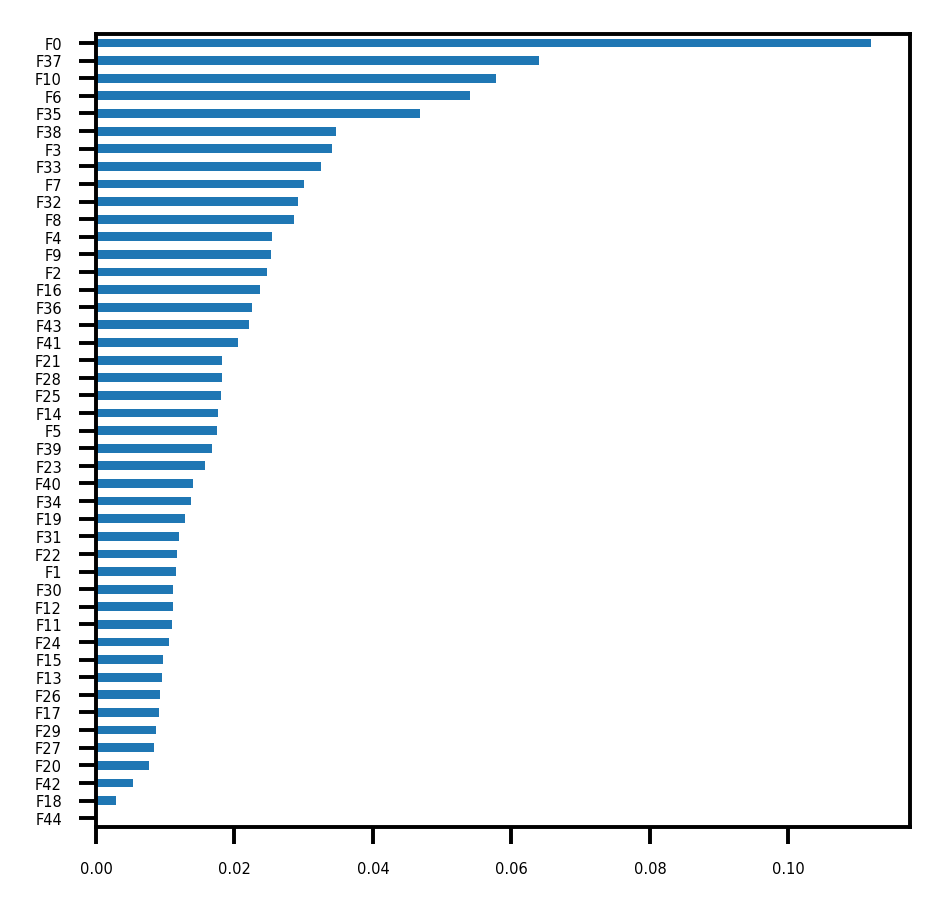
\includegraphics[width=0.45\textwidth,height=90mm]{assets/feature_importances.png}
  \\ Fonte: Condução dos experimentos pelos autores do artigo.
\end{figure}

% \def\code#1{\texttt{#1}}
% \code{\small{RandomForestClassifier}}

\subsection{Resultados dos modelos em Validação}

Tabela 3: Resultados dos Modelos em Validação
\begin{center}
\begin{tabular}{lr}

    \Xhline{2.5\arrayrulewidth}
    \textbf{Classificador} &         \textbf{KS} \\
    \Xhline{2.5\arrayrulewidth}

    \textit{RandomForestClassifier} &  20.730660 \\
    \hline
    \textit{XGBClassifier} &  \textbf{26.341257} \\
    \hline
    \textit{AdaBoostClassifier} &  25.197695 \\
    \hline
    \textit{LogisticRegression} &  18.471405 \\
    \hline
    \textit{LGBMClassifier} &  \textbf{27.209834} \\

\end{tabular}
\\ Fonte: Condução dos experimentos pelos autores do artigo.
\end{center}

Acerca do teste dos modelos \textit{XGBClassifier} e \textit{LGBMClassifier}, obtemos como resultado (KS), respectivamente, 27.1 e 26.9.